\documentclass[12pt]{article}

\usepackage[T2A]{fontenc}
\usepackage[utf8]{inputenc}
\usepackage[english,russian]{babel}

\usepackage[T2A]{fontenc}
\usepackage[utf8]{inputenc}
\usepackage[russian]{babel}

\usepackage[
    a4paper,
    left=3cm,
    right=2cm,
    top=2cm,
    bottom=2cm
]{geometry}

%% Figures
\usepackage{tkz-euclide}
\usepackage{subcaption}
\usepackage{amsmath}
\usepackage{amssymb}

%% Hyphenation rules
\usepackage{hyphenat}

\usepackage[hidelinks]{hyperref}

%%colorfull
\usepackage{xcolor}

\usepackage{indentfirst}

\usepackage{graphicx}

\DeclareGraphicsExtensions{.pdf,.png,.jpg}
\graphicspath{ {pic/} }
% Настройка списков
\usepackage{enumitem}
\setlist{nolistsep, labelsep=0.4cm, leftmargin=1.85cm}

% Красная строка у первого абзаца посе заголовка
% (по умолчанию не ставится)
\usepackage{indentfirst}

% Здесь укажите свойства
\linespread{1.15}
\parindent = 0.75cm

\begin{document}

\section{Фракталы}

\textbf{Фрактал} (лат. fractus - дроблёный, сломаный, разбитый) - множество, обладающее свойством самоподобия (объект, в точности или приблежённо совпадающий с частью себя самого, то есть целое имеет ту же форму что и одна или более частей).
\begin{figure}[h!]
    \centering
    
\includegraphics[width=0.5\textwidth]{10-1-1}
    \caption{\small Множество Мандельброта}
\end{figure}
\subsection{Фракталы в природе}
В живой природе:

\begin{itemize}
    \item кораллы;
    \item морские звезды, ежи, раковины;
    \item цветы и растения (брокколи, капуста);
    \item кроны деревьев и листья растений (см. рис. 3);
    \item кровеносная системы и бронхи людей и животных.
\end{itemize}
\begin{figure}[h!]
    \centering
    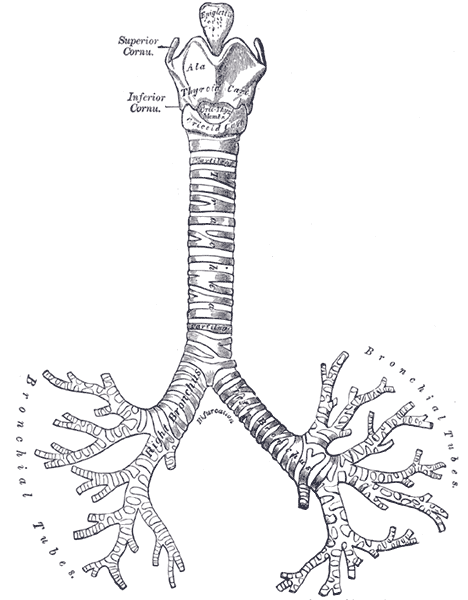
\includegraphics[height=0.5\textwidth]{10-1-3}
    \caption{\small Бронхи человека}
\end{figure}
В неживой природе:
\begin{itemize}
    \item границы георафических объектов (стран, областей, городов);
    \item береговые линии;
    \item горные хребты;
    \item снежинки;
    \item облака;
    \item кристаллы (например, кристалл висмута, рис 3).
\end{itemize}
\begin{figure}[h!]
    \centering
    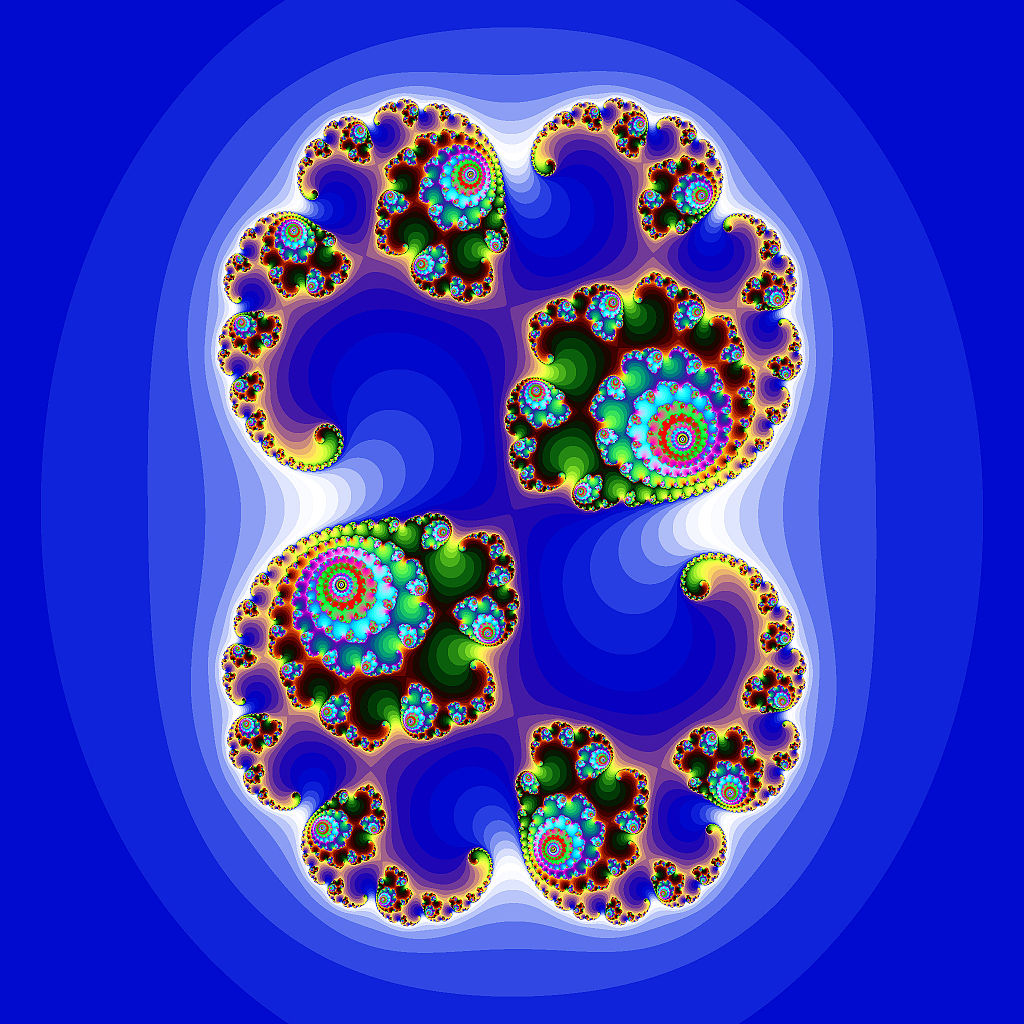
\includegraphics[width=0.5\textwidth]{10-1-2}
    \caption{\small Множество Жюлиа}
\end{figure}
\end{document}